%kelompok 1 Sistem Operasi (Semaphore)
%Kelas D4 TI 1B
%Adam Noer Hidayatullah 1174097
%Ichsan Hizman
%Teddy
%Nisrina Aulia
%Irvan Rizkiansyah 1174043

\section{proses}

	\subsection{Proses}	
	Proses adalah sebuah  program yang sedang dieksekusi. Sedangkan program idalah merupakan kumpulan-kumpulan  dari suatu  instruksi yang sudah ditulis ke dalam bahasa yang dapat  dimengerti oleh sistem operasi.Proses berisi tentang sebuah instruksi dan sebuah data. program counter dan seluruh register pemroses, stack ini  berisi data sementara contohnya seperti alamat pengiriman, parameter rutin dan variabel lokal. Sistem operasi diharuskan untuk mengelola semua proses di dalam sistem tersebut dan mengalokasikan sumber daya ke sebuah  proses-proses sesuai dengan kebijaksanaan untuk memenuhi sasaran sistem
	
	\subsection{Istilah yang berkaitan dengan proses}
		\begin{itemize}
			\item Multiprogramming
			Multiprogramming (multitasking) adalah  istilah teknologi informasi dengan mengunakan bahasa inggris yang baik  mengacup kepada sebuah metode dimana banyak sebuah pekerjaan atau yang dikenal juga sebagai proses  dengan diolah dengan menggunakan sumber daya CPU yang sama.
			Contohnya sistem operasi jenis ini antaranya linux dan windows.
			\item Multiprocessing
			kemampuan komputer untuk melakukan beberapa proses dengan waktu yang bersamaan, dibantu dengan keberadaan teknologi yang berbasis multiprocessor.
			Contohnya seperti computer server.
			\item Distributed processing/computing
			Mengerjakan semua proses pengolahan data secara bersamaan antara komputer pusat dengan beberapa komputer yang lebih kecil dan saling berhubungan denan melalui jalur komunikasi.
			Contohnya komputer yang dirancang untuk melaksanakan tugas-tugas proyek.
		\end{itemize}
		
	\subsection{Fungsi fungsi sistem operasi}
		\begin{enumerate}
			\item Resource manager, pengolahan sumber daya dan mengalokasikan.
			\item Interface atau tatap muka, sebagai perantara antara pengguna dengan perangkat keras.
			\item Coordinator, mengkoordinasi fasilitas sehingga aktifitas yang komplek dapat diatur..
		\end{enumerate}
		
		\subsection{jenis jenis sistem operasi pada komputer}
			\begin{enumerate}
				\item Windows, merupakan pengembangan dari sistem operasi DOS. windows juga mudah untuk dipelajari.
				\item Mac OS, merupakan sistem operasi yang diciptakan oleh Apple. Mac OS memiliki tingkat keamanan yang tinggi.
				\item Linux, memiliki kestabilan yang baik, yang sering digunakan sebagai sistem operasi pada server.
				\item Android, merupakan sistem operasi pada smartphone. android sama seperti Linux, yaitu mudah dikembangkan.
			\end{enumerate}
			
	\subsection{Status proses}
	Terdapat 5 macam jenis status yang mungkin dimiliki oleh suatu proses :
	\begin{enumerate}
		\item New, yaitu status yang dimiliki pada saat proses baru saja terjadi.
		\item Ready, yaitu status dimana proses siap untuk dieksekusi pada giliran berikutnya.
		\item Running, yaitu status suatu proses dimana saat ini proses tersebut sedang dieksekusi oleh prosesor
		\item Waiting, yaitu status dimana proses yang tidak bisa dijalankan di saat prosesor sudah siap, status yang dimiliki pada saat proses menunggu suatu sebuah event seperti I/O
		\item Terminated, yaitu status yang dimiliki pada saat proses telah selesai dieksekusi
	\end{enumerate}
	
	Berikut ini adalah proses dari ke-5 status proses di atas :
	\begin{enumerate}
		\item New ke Ready
		Pertama Status dibuat lalu setelah itu , status akan memasuki proses ready dan siap untuk memasuki proses selanjutnya.
		\item Ready ke running
		Di saat sedang memilih proses yang akan dioperasikan, sistem operasi akan memilih salah satu proses yang berada didalam keadaan status ready.
		\item Running ke waiting
		Suatu proses dimasukkan dalam keadaan status waiting jika proses itu meminta sesuatu yang dapat menyebabkannya harus menunggu. Sebuah request ke sistem operasi yang pada umumnya merupakan bentuk panggilan dari layanan sistem (panggilan dari program yang sedang beroperasi ke dalam suatu prosedur yang merupakan bagian kode sistem operasi) misalnya seperti sebuah proses yang bisa meminta suatu layanan dari sistem operasi yang tidak siap dilakukan oleh sistem opersi dengan segera. Atau proses yang bisa menginisiasi suatu aksi, seperti misalnya operasi I/O, yang seharusnya bisa diselesaikan sebelum proses itu melanjutkan operasinya. Pada saat proses saling melakukan komunikasi dengan proses yang lainnya, suatu proses bisa diblokir jika sedang menunggu proses lainnya untuk menyediakan input.
		\item Running ke ready
		Pada umumnya alasan transisi ini ialah dimana sebuah proses yang lagi berjalan sudah mencapai batas waktu maksimum yang telah diizinkan bagi instruksi yang tidak diinterupsi. Terdapat beberapa alasan yang menyebabkan transisi ini terjadi, yang tidak diimplementasikan oleh setiap sistem operasi. Misalnya apabila sistem operasi meng-assign tingkat prioritas yang berbeda pada beberapa proses yang berlainan, suatu proses bisa diambil lebih dulu.
		\item Waiting ke ready
		Apabila suatu proses dalam keadaan status waiting sudah selesai dalam mendapatkan sumber daya, seperti file atau bagian virtual memori bagi pakai atau juga sudah selesai setelah menunggu proses yang lainnya untuk menyediakan input atau sudah selesai dalam menunggu pesan lainnya.
		\item Runing ke finish(terminated)
		proses yang sedang berjalan dihentikan oleh Sistem Operasi jika proses itu telah selesai atau tidak jadi dieksekusi. Hal ini terjadi dikarenakan jika proses induknya sendiri telah berhenti.
	\end{enumerate}
	
	Dan berikut ini adalah diagram dari ke-5 status proses tadi :
	
	\begin{figure} [ht]
	\centerline{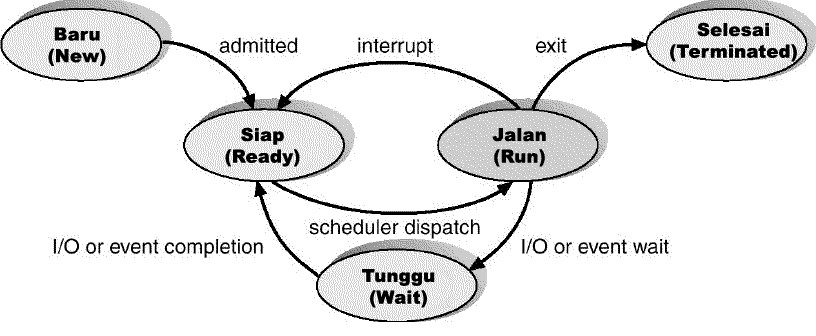
\includegraphics[width=1\textwidth]{figures/statusproses.jpg}}
	\caption{Gambar Status Proses}
	\label{statusproses}
	\end{figure}
	
	\ref{statusproses}
	
	\subsection{Contoh dari status proses}
	Setiap proses pasti mempunyai status yang harus diperhatikan oleh sistem operasi yang akan dicatat dalam berbagai macam tabel yang saling berhubungan, yaitu :
		\begin{itemize}
			\item Tabel informasi manajemen memori, Digunakan untuk menjaga keutuhan dari suatu memori utama dan memori sekunder yang akan menyimpan suatu informasi.
			\item Tabel informasi manajemen masukan atau keluaran, Digunakan untuk melakukan pengelolan sebuah perangkat masukan atau keluaran, yang dimana perangkat tersebut akan digunakan oleh proses yang tertentu, sehingga harus dijaga supaya proses yang lainnya tidak akan memakainya. Sistem operasi harus mengetahui status operasi masukan atau keluaran dan lokasi suatu memori utama yang akan digunakan untuk melakukan transfer data.
			\item Tabel informasi sistem file, Tabel dimana yang berisikan mengenai informasi lokasi pada memori sekunder, informasi ekstensi file, informasi status pada saat itu dan menyimpan atribut-atribut file yang lainnya.
			\item Tabel proses, Digunakan untuk mengelola informasi suatu proses pada sistem operasi, yang berlokasi di memori, atribut proses dan status lainnya.
		\end{itemize}
	
	\subsection{Proses Control Block/Blocked}
	Sebuah struktur data yang dipakai oleh Sistem Operasi untuk mengelola sebuah proses. Hampir semua Sistem Operasi yang modern telah menggunakan PCB (Process Control Block) namun strukturnya yang berbeda-beda pada setiap Sistem Operasi tersebut. PCB (Process Control Block) juga memiliki informasi yang berhubungan dengan proses, ialah: tanda pengenal bagi sebuah proses (Process ID) yang sangat unik dan akan menjadi status proses, nomor identitas, prioritas eksekusi proses dan semua informasi lokasi proses dalam memori. Prioritas yang dimiliki oleh sebuah proses merupakan sebuah nilai atau besaran yang akan menunjukkan seberapa sering proses harus dieksekusi oleh prosesor. Sebuah proses yang mempunyai nilai prioritas yang cenderung lebih tinggi, akan lebih sering dieksekusi atau dieksekusi terlebih dulu jika dibandingkan dengan proses yang mempunyai prioritas yang lebih rendah.
	Sebuah PCB (Process Control Block) ditunjukkan dalam tabel berikut : 
	
	\begin{table}[H]
		\begin{tabular}{|c|c|}
			\hline
			Pointer & State Proses\\
			\hline
			\multicolumn{2}{|c|}{Nomor Proses}\\
			\hline
			\multicolumn{2}{|c|}{Program Counter}\\
			\hline
			\multicolumn{2}{|c|}{Registers}\\
			\hline
			\multicolumn{2}{|c|}{Batas Memori}\\
			\hline
			\multicolumn{2}{|c|}{Daftar berkas yang telah dibuka}\\
			\hline
			\multicolumn{2}{|c|}{.......}\\
		\end{tabular}
	\end{table}
	
	PCB dibagi menjadi 3 kelompok yaitu :
	\begin{itemize}
		\item Process identification data
		pasti akan selalu mengikut-sertakan suatu identifier yang sangat unik untuk prosesnya (hampir selalu mempunyai nilai integer) dan pada sebuah sistem multiuser-multitasking, data yang contohnya seperti identifier grup pengguna, identifier proses, identifier pengguna, dan yang lainnya. Proses ini sangat relevan, karena itu sering dipakai untuk referensi silang tabel sistem operasi, misalnya seperti memungkinkan untuk mengidentifikasi sebuah proses yang menggunakan device I/O, atau daerah memori.
		\item Processor state data
		potongan-potongan dari informasi yang mengartidefinisikan status dari sebuah proses ketika proses tersebut ditangguhkan, dan memungkinkan sistem operasi untuk melakukan restart proses pada akhirnya dan akan masih dapat mengeksekusinya dengan benar. Hal ini akan selalu mengikut-sertakan isi dari register CPU tujuan.
		\item Process control data
		digunakan oleh sistem operasi untuk mengelola proses itu sendiri.
	\end{itemize}
Dirangkum dari makalah \cite{apriyanto2009sistem}
Dirangkum dari makalah \cite{silberschatz2014operating}